\documentclass[11pt,a4paper]{article}

\usepackage{graphicx}
\usepackage{subcaption}
\usepackage{float}
\usepackage[utf8x]{inputenc}
\usepackage[greek,english]{babel}
\usepackage{amsthm, amssymb, amsmath, centernot}
\usepackage{mathrsfs}
\newcommand{\notimplies}{%
  \mathrel{{\ooalign{\hidewidth$\not\phantom{=}$\hidewidth\cr$\implies$}}}}
\renewcommand{\d}[1]{\mathrm{d}#1}
\newcommand{\deriv}[2]{\frac{\d{#1}}{\d{#2}}}
\newcommand{\pderiv}[2]{\frac{\partial{#1}}{\partial{#2}}}
\newcommand{\cderiv}[3]{\left(\frac{\partial{#1}}{\partial{#2}}\right)_{#3}}
\renewcommand\qedsymbol{$\square$}
\newcommand{\cont}{$\boxtimes$}
\newcommand{\divides}{\mid}
\newcommand{\ndivides}{\centernot \mid}
\newcommand{\Z}{\mathbb{Z}}
\newcommand{\N}{\mathbb{N}}
\newcommand{\C}{\mathbb{C}}
\newcommand{\Zplus}{\mathbb{Z}^{+}}
\newcommand{\Primes}{\mathbb{P}}
\newcommand{\ball}[2]{B_{#1} \! \left(#2 \right)}
\newcommand{\Q}{\mathbb{Q}}
\newcommand{\R}{\mathbb{R}}
\newcommand{\Rplus}{\mathbb{R}^+}
\newcommand{\invI}[2]{#1^{-1} \left( #2 \right)}
\newcommand{\End}[1]{\text{End}\left( A \right)}
\newcommand{\legsym}[2]{\left(\frac{#1}{#2} \right)}
\renewcommand{\mod}[3]{\: #1 \equiv #2 \: \mathrm{mod} \: #3 \:}
\newcommand{\nmod}[3]{\: #1 \centernot \equiv #2 \: mod \: #3 \:}
\newcommand{\ndiv}{\hspace{-4pt}\not \divides \hspace{2pt}}
\newcommand{\finfield}[1]{\mathbb{F}_{#1}}
\newcommand{\finunits}[1]{\mathbb{F}_{#1}^{\times}}
\newcommand{\ord}[1]{\mathrm{ord}\! \left(#1 \right)}
\newcommand{\quadfield}[1]{\Q \small(\sqrt{#1} \small)}
\newcommand{\vspan}[1]{\mathrm{span}\! \left\{#1 \right\}}
\newcommand{\galgroup}[1]{Gal \small(#1 \small)}
\newcommand{\sm}{\! \setminus \!}
\newcommand{\topo}{\mathcal{T}}
\newcommand{\base}{\mathcal{B}}
\renewcommand{\bf}[1]{\mathbf{#1}}
\renewcommand{\Im}[1]{\mathrm{Im} \: #1}
\renewcommand{\empty}{\varnothing}
\renewcommand{\th}[1]{$#1^\mathrm{th}$}

\newenvironment{definition}[1][Definition:]{\begin{trivlist}
\item[\hskip \labelsep {\bfseries #1}]}{\end{trivlist}}

\theoremstyle{theorem}
\newtheorem{theorem}{Theorem}[section]
\newtheorem{lemma}[theorem]{Lemma}

\theoremstyle{definition}
\newtheorem*{problem}{Problem}

\theoremstyle{definition}
\newtheorem*{proposition}{Proposition}

\theoremstyle{remark}
\newtheorem*{fact}{Fact}

\theoremstyle{definition}
\newtheorem{example}{Example}[section]

\theoremstyle{remark}
\newtheorem{remark}{Remark}[subsection]


\newcommand{\phase}{\mathscr{X}}

\begin{document}
\author{Benjamin Church}
\title{\Huge Introduction to Statistical Mechanics}

\maketitle
\tableofcontents
\newpage


\section{Introduction}
Even in simple cases, Newton's laws for a single particle can be difficult to solve exactly. If we increse the number of particles, the difficulty rapidly increases even further. Famously, there is no exact known solution to the problem of three particles moving under the influces of eachothers gravity known as the three body problem. Such relatively small mechanics problems stumped the greatest minds of the \th{17} and \th{18} centuries from Euler to Lagrange to Jacobi. The task of predicting the properties from first principles of a real material made from trillions of trillions of interacting atoms seemed entirely impossible. However, it turns out that a huge amount of information about macroscopic properties can be learned while knowing almost nothing about the exact microscopic movements and behaviors. The trick of statistical mechanics is to shift the goal posts, to change the question. It is true that nobody will ever be able to write down a solution to Newton's laws (or even less likely to the Schr{\"o}dinger equation) for thousands of interacting atoms let alone the myriads that makeup the tinyies visible object. However, we can determine the average behavior and bulk properties. Calling upon the law of large numbers, the exact issue that made solving the system so difficult, the number of particles involved, now becomes our greatest stregnth. As the number of particles becomes greater, average behavior becomes closer and closer to the exact real behavior.

\section{Phase Space and Statistical Ensembles}     
In this section we will discuss some helpful notation and terminology for talking about statisical mechanics. The ideas here are very simple so try to not lose them amoung the fancy words. \bigskip \\
The most convient method for keeping track of everything one needs to know about a physical system is to track its position in phase space which I will denote as $\phase$. Phase space is defined such that each point uniquely represents any possible state for the system to be in. For example, the phase space of a single particle constrained to move in one-dimension is a two-dimensional space defined by the pair ($q$, $p$) of position $q$ and momentum $p$ (often refered to as $q-p$ space). In general, a system of $N$ particles in three dimensions is a $6 N$ dimensional space with three dimensions for the position of each particle and three dimensions for the momentum of each particle. There are good reasons why momentum is the prefered quantity over velocity to define phase space but the reasons are due to the Hamiltonian formulation of mechanics which is somewhat beyond the scope of this class. If you are interested, ask me after class or shoot me an email. The phase spaces I have defined so far are all continuous, however, we can also consider a discrete phase space corresponding to a system with a discrete set of possible states. Such phase spaces often come up in quantum mechanics in which the set of possible states is \textit{quantized}, that is, discrete. Another way discrete phase spaces pop up is as an approximation to some continuous system. For example, we can model an electron moving in a lattice of tighly binding nuclei as only having possible states, the electron is closesly bound to this partucular atom, as opposed to the more accurate view that there is a continuum of position states for the electron between atoms. However, if the interactions are very strong and the distance between atoms is small, this approximation can be very accurate and useful. From here on, I will refer to a point in phase space, that is a state of the system, as a microstate. \bigskip\\
A statistical ensemble is a probability distribution over the phase space of a system. All this means is that a statistical ensemble is a set of possible states the system could be in each weighted by the probability of it being in that state. Since the properties and evolution of a single microstate are too difficult to work out, we will spend our effort on discussing the properties of an entire ensemble of microstates which is surprisingly much easier. One of the reasons ensebles are so important is that they give us a way to talk about thermodynamic equilibrium in which the temperature of the entire system equilibrates. But what does thermodynmaic equilibrium really mean and for that matter what does temperature really mean?

\section{Entropy and Temperature}

\subsection{What is Entropy?}

The most fundamental quantity in statistical mechanics (perhaps besides energy) is entropy. Entropy is often described as a measure of disorder or chaos but that is somewhat misleading. The real definition of entropy is a measure of uncertainty about the microstate of a system given a macrostate or ensemble. In essense, entropy measures how many different microstates perfectly reproduce a particular macrostate. There are many equivalently messy ways to be disordered yet very few ways to be equivalently ordered. Therefore, a disorderly macrostate will often have higher entropy than an ordered one. For example, there are many more possible random combinations of water mollcules in a fluid which all look macroscopically identical than there are ordered arrangements of water mollecules in an ice crystal. This is why entropy and disorder are often conflated. 

\subsection{The Microcanonical Ensemble}



\subsection{Defining Temperature}

One piece of information about the macrostate we might have is the total energy of the system. This situation is sufficiently important for us to consider it in depth here. In statistical mechanics, we often have a family of probability distributions parametrized by the total energy, that is, a function $P(X;E)$ both of a variable $X$ in phase space and $E$ the total energy. In this case, we can consider the entropy as a function of energy $S_P(E) = S[P(E)]$. Now we will make a remarkable and probably baffeling definition. I define the temperature $T$ of a family of distributions $P$ by the equation,
\[ \frac{1}{T} = \deriv{S_P(E)}{E} \]
It will not at all be clear why this is a sensible definition until the next section. However, it may now be clear why the factor $k_B$ is often included in the definition of the entropy. This factor makes the quantity $\deriv{S_p(E)}{E}$ have units of inverse temperature.

\subsection{An Example: the Two State System}

\subsection{The Entropy of a Probability Distribution}

Since a statistical ensemble is nothing more than a probability distribution, we should define the entropy (think uncertainty) of a probability distribution. We want entropy to satisfy a few fundamental properties. 
\begin{enumerate}
\item $S[P] \ge 0$ for any probability distribution $P(X)$ with $X \in \phase$.

\item $S[\delta_{X_0}] = 0$ where $\delta_{X_0} = 1$ if $X = X_0$ and $\delta_{x_0}(x) = 0$ otherwise. In other words, the distribution corresponding to a single definite state has zero entropy.

\item $S[P_1 \cdot P_2] = S[P_1] + S[P_2]$ where $P_1 \cdot P_2$ is the probability distribution defined by $P_1 \cdot P_2 (X) = P_1(X) \cdot P_2(X)$ for any $X \in \phase$. That is, the entropy of a ensemble which can be decomposed into two independent parts is the sum of the parts.  
\end{enumerate}
It turns out that these properties are enough to nearly fix the form of $S$. Given a distribution on the phase space $\phase$, we can take the entropy to be,
\[ S[P] = - k \sum_{X \in \phase} P(X) \log{P(X)} \]
The form of this function is determined upto the overall constant. It is conventional to either set $k = 1$ or $k = k_B = 1.380648 \cdot 10^{-23} \: \mathrm{J} \: \mathrm{K}^{-1}$ the Boltzmann constant which should be thought of as a conversion factor between Joules (macroscopic units of energy) and Kelvin (microscopic units of energy). Although these are the only conventions used in practice, it is good to remember that the constant here is arbitrary and therefore cannot change any of the underlying physics. 
When dealing with a continuuous phase space, it is natural to replace the sum by an integral \footnote{There is a subltly here with the distiction between a continuous and discrete phase space. This formula is correct for a discrete phase space. The natural generalization to a probability densitiy function over a continuuous phase space of switching the sum to an integral almost works perfectly. This prescription actually shifts the value of the entropy by a constant which allows the continuous version to be negative. We will not deal with this difficulty here since it does not affect any of the conclusions.} over the probability densitiy such that the entropy becomes,
\[ S[P] = -k \int_{\phase} \d{X} \: f(X) \log{f(X)} \]
where $f$ is a probability density function.
Although this definition may seem mysterious, the idea is quite simple and important to remember. Entropy measures how uncertian we are about the microstate given information about the macrostate.


\section{The Second Law of Thermodynamics}

So far I have only given you definitions but nothing of actual physical content. To start, we will need some axiom, some physical assumption to kcikstart our study and link these abstract concepts to physical reality. The foundational assumption is known as the second law of thermodynamics which states,
\begin{center}
\textit{The entropy of a closed system never decreases and increases whenever possible.}
\end{center}
and the very important (alhtough rarely quoted) corollary,
\begin{center}
\textit{A system has reached thermodynamic equilibrium when its entropy is maximized keeping other parameters (for example energy) held fixed.} 
\end{center}
This corollary follows because if a system has not reached its maximum entropy then it must, by all reason, be able it increase its entropy and therefore, by the second law, it will which will spontaneously change macroscopic parameters (think ice melting). If you wish, you may take this corollary as the definition of thermodynamic equilibirum. 

\subsection{The Flow of Heat}

Suppose we can divide our system into two parts $A$ and $B$ which can transfer energy between them. Consider a small transfer of energy (called heat) $\Delta Q$ from $B$ to $A$. The change of entropy durring this process is then,
\[ \Delta S_{tot} = \Delta S_A + \Delta S_B = \Delta Q \deriv{S_A}{E} + (- \Delta Q) \deriv{S_B}{E} = \frac{\Delta Q}{T_A} - \frac{\Delta Q}{T_B} \]
By the second law, we know that this process will only occur in nature when $\Delta S_{tot} \ge 0$. Therefore,
\[ \Delta Q \left( \frac{1}{T_A} - \frac{1}{T_B} \right) \ge 0\]
which, since $\Delta Q$ is by definition a positive quantity, implies that 
\[ T_A \le T_B \]
Therefore, heat will only flow from $B$ to $A$ when then temperature of $A$ is less than the temperature of $B$. This is the fundamental property of temperature, heat folows from hot to cold. The fact that our quantity $T$ satisfies this important property of a measure of temperature justifies this as a good definition of temperatue.

\subsection{Justifying the Second Law}

The second law is extremely fundamental. However, using some physical reasoning about the behaviors of large numbers of particles, we can justify why it might be true (GIVE JUST).

Although the second law  may seem like an \textit{ad hoc} assumption, this is truly the cornerstone upon which all of statistical mechanincs, thermodynamics, and chemisty rests. In fact, once  the second law becomes natural, it is surprising just how little we need to assume and just how much follows formally from this physical assumption. 

\subsection{Reversibility and Irreversibility}

\subsection{The Arrow of Time}

\subsection{What It All Means}

In the modern view, the second law is a \textit{statistical} law rather than an absolute one. In other words, the second law does not need to hold exactly every time. For a system of a small number of particles, there is a finite probability of spontaneous ordering into a state with few permutations and therefore lower entropy. Furthermore, if there are a small enough number of particles that we can accurately track the exact state of the system the whole concept of entropy makes little sense! However, the second law holds in the thermodynamical limit as the number of particles grows $N \to \infty$. As we increse the number of particles, the probability of violating the second law by spontaneously decreasing the entropy becomes vanishingly small. For a system with $N \sim 10^{23}$ the probability of macroscopically decreasing the entropy is essentially zero! It is very much akin to expecting glass shards when thrown against a wall to spontaneously form a wine-glass. Not techincally impossible by the known microscopic laws of physics but truly \textit{impossible} by any practical sense of the word. The slightly fuzzy, inexact nature of the second law should not disuade you from its power and ushakable certianty as a foundational pillar of modern physics. I will leave you with a quote from the legendary astrophysicst Sir Arthur Eddington who was the first to experimentally verify Einstein's theory of General Relativity and also coined the term ``arrow of time'', 

\begin{quote}
The law that entropy always increases, holds, I think, the supreme position among the laws of Nature. If someone points out to you that your pet theory of the universe is in disagreement with Maxwell's equations -- then so much the worse for Maxwell's equations. If it is found to be contradicted by observation -- well, these experimentalists do bungle things sometimes. But if your theory is found to be against the second law of thermodynamics I can give you no hope; there is nothing for it but to collapse in deepest humiliation.
\end{quote}


\section{The Boltzmann Distribution}

\subsection{The Canonical Ensemble}

At last, we will dive into the meat of the subject. (DESCRIBE CANONICAL ENSEMBLE) Following the second law, to find the statistical ensemble for a system in thermodynamic equilibrium, we should try to maximize the entropy of the ensemble subject to the contraint of a fixed average energy. To do this, we will use Lagrange multipliers. (see Appendix A.) For this illustration, we will assume that our phase space $\phase$ is discrete but the same idea will hold in general. We want to maximize the function\footnote{I have dropped the factor of $k_B$ here for notational simplicity. Here, this factor makes no difference since maximizing any positive multiple of a function is the same as maximizing the origional function.},
\[S[P] = - \sum_{X \in \phase} P(X) \log{P(X)} \]
subject to the constraints that the expected energy is some fixed value $E$ and that the total probability adds up to $1$ (which better be true if we want to call it a probability distribution). These constraints are,
\[ F[P] = \sum_{X \in \phase} P(X) = 1 \quad \text{and} \quad G[P] = \sum_{X \in \phase}  P(X) \cdot E(X) = E \]
Using Lagrange multipliers, we set, the derivatives with respect to each variable proportional,
\[ \pderiv{S[P]}{P(X)} = \alpha \pderiv{F[P]}{P(X)} + \beta \pderiv{G[P]}{P(X)} \]
which becomes,
\[ - \log{P(X)} - 1 = \alpha + \beta E(X) \]
which immediately implies that,
\[ P(X) = e^{-(1 + \alpha)} \cdot e^{- \beta E(X)} \]
Since $\alpha$ is an arbitrary parameter which will be fixed later, we may define for notational simplicity,
\[ \frac{1}{Z} = e^{-(1 + \alpha)} \]
such that the result becomes,
\[ P(X) = \frac{1}{Z} e^{-\beta E(X)} \]
This is the fundamental form of the most important probability distribution in physics: the Boltzmann distribution. In the next section, we will explore the meaning of the, as yet, undetermined constants $Z$ and $\beta$.

\subsection{The Partition Function and Free Energy}

It it important to remember that, by definition, these constants $\alpha$ or $Z$ and $\beta$ are universal to the macrostate of the system; they do not depend on the microstate $X$. Now we need to determine these coeficients. By using the constraint $F[P] = 1$, we get,
\[ \sum_{X \in \phase} P(X) = \sum_{X \in \phase} \frac{1}{Z} e^{-\beta E(X)} = 1\]
which implies that,
\[ Z = \sum_{X \in \phase} e^{-\beta P(X)}\]
The quantitiy $Z$ is called the partition function. We will find that everything we might ever want to know about macroscopic properties is contained in $Z$. To fix the constant $\beta$, we should calculate the energy and entropy of this family of distributions $P(X;\beta)$. 
\begin{align*}
E & = \sum_{X \in \phase} P(X; \beta) E(X) = \frac{1}{Z} \sum_{X \in \phase} E(X) e^{-\beta E(X)} = - \frac{1}{Z} \sum_{X \in \phase} (-E(X)) e^{-\beta E(X)}
\\
& = -\frac{1}{Z} \deriv{}{\beta} \left[ \sum_{X \in \phase} e^{-\beta E(X)} \right] = - \frac{1}{Z} \deriv{Z}{\beta} = - \deriv{\log{Z}}{\beta} 
\end{align*}
so we see the first inclination that the partition function is important, its logarithmic derivative gives the energy of the system. Furthermore,
\begin{align*}
S[P] &= - k_B \sum_{X \in \phase} P(X;\beta) \log{P(X;\beta)} = - k_B \sum_{X \in \phase} P(X;\beta) \log{\left[ \frac{1}{Z} e^{-\beta E(X)} \right]} 
\\
&= k_B \sum_{X \in \phase} P(X; \beta) \left[\beta E(X) + \log{Z} \right] = k_B  \beta \sum_{X \in \phase} P(X;\beta) E(X) + k_B \log{Z} \cdot \sum_{X \in \phase} P(X;\beta) 
\\
& = k_B \beta E + k_B \log{Z}
\end{align*}
Now consider the derivative,
\begin{align*}
\deriv{S(E)}{E} & = k_B \beta + k_B \deriv{\beta}{E} E + k_B \deriv{\log{Z}}{E} = k_B \beta + k_B \deriv{\beta}{E} E + k_B \deriv{\log{Z}}{\beta} \deriv{\beta}{E} 
\end{align*}
which, using the above formula for the energy becomes,
\[\deriv{S(E)}{E} = k_B \beta + k_B \deriv{\beta}{E} E - k_B E \deriv{\beta}{E} = k_B \beta \]
Therefore, our definition of temperature sets,
\[ \frac{1}{T} = k_B \beta \implies \beta = \frac{1}{k_B T} \]
Therefore, the equilibrium statistical ensemble becomes,
\[ P(X) = \frac{1}{Z} \: e^{-\tfrac{E(X)}{k_B T}} \quad \text{where} \quad Z = \sum_{X \in \phase} e^{-\tfrac{E(X)}{k_B T}} \]
which is the famous Boltzmann distribution. This distribution is simply beautiful due to its marvelous simplicity and, as we will shortly see, breathtaking power and applicability. \bigskip\\
I will end this section by rewriting the formula we derived above for the entropy as,
\[ S[P] = \frac{1}{T} E + k_B \log{Z} \]
and therefore,
\[ E = TS - k_B T \log{Z} \]
The quantity,
\[ F = E - TS = -k_B T \log{Z} \]
will be sufficiently important to get a fancy name. We call $F$ the Helmholtz free energy. We will see that $F$ somehow encodes the amount of ``usable'' work one can extract from a system. This quantity will show up again and again.

\section{Examples of Equilibrium Thermodynamics}

Although it may not seem like it, we have now worked out the majority of the theory behind statistical mechanics. What is left is to calculate its consequences in whatever physical system suits our fancy.

\subsection{Lattice in a Gravitational Field}

Consider a one-dimensional lattice of atoms which can tightly bind electrons. Suppose the lattice is verticle so that the gravitational potential energy increases as we go up the lattice. If we use the tight-binding approximation in which electrons are always bound to a single atom and we also neglect the interactions between electrion, then the energy of a state is simply,
\[ E(X) = \sum_{i = 1}^N mgd x_i \]
where $x_i$ is the position (along the lattice) of the \th{i} electron, $N$ is the total number of electrons, $m$ is the mass of an electron, and $d$ is the lattice spacing. Therefore, the partition function becomes,
\[ Z = \sum_{x_i \in \N} e^{-\beta \sum\limits_{i = 1}^N mgd x_i} = \left[ \sum_{n = 0}^\infty e^{-n(\beta mg d)} \right]^N = \left(\frac{1}{1 - e^{-\beta m g L}} \right)^N \]
Therefore, 
\[\log{Z} = - N \log{1 - e^{-\beta mg d}} \]
so using our general formula,
\[ E = - \deriv{\log{Z}}{\beta} = N mgd \frac{e^{-\beta m g d}}{1 - e^{-\beta m g d}} = \frac{N mg d}{e^{\frac{mgd}{k_B T}} - 1} \]
\begin{figure}
\begin{center}
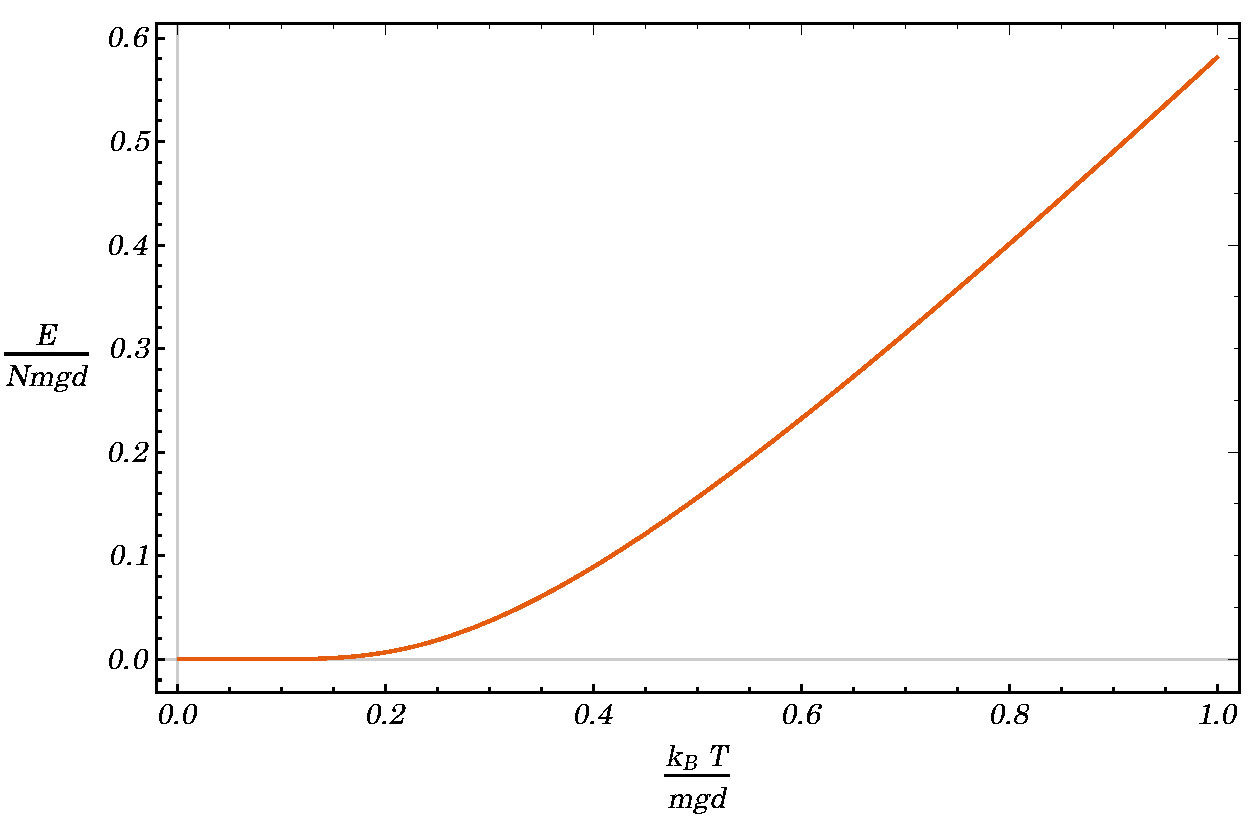
\includegraphics[width = 9cm, height = 6cm]{GravLatticeEnergy}
\caption{The energy-temperature relationship for a one-dimensional lattice in a gravitational field.}
\label{energygravlattice}
\end{center}
\end{figure}
The energy dependence can be understood in two regimes based on a critical or cutoff temperature, $T_c = \frac{mgd}{k_B}$. When $T \gg T_c$ then we can expand $e^{T_c/T} \approx 1 + T_c/T$ and therefore,
\[ E \approx \frac{N mg d}{1 + T_c/T - 1} =  \frac{N mgd}{T_c} T = k_B T \]
In the high temperature (much greater than critical) regime the energy grows approximatly linearly with temperature. On the other hand, at low temperature, $T \ll T_c$ we have the opposite situation, $T_c/T \gg 1$ so $e^{T_c/T} \gg 1$ and therefore,
\[ E = \frac{N mg d}{e^{T_c/T} - 1} \approx N mgd \cdot e^{-T_c/T} \]
\begin{figure}
\begin{center}
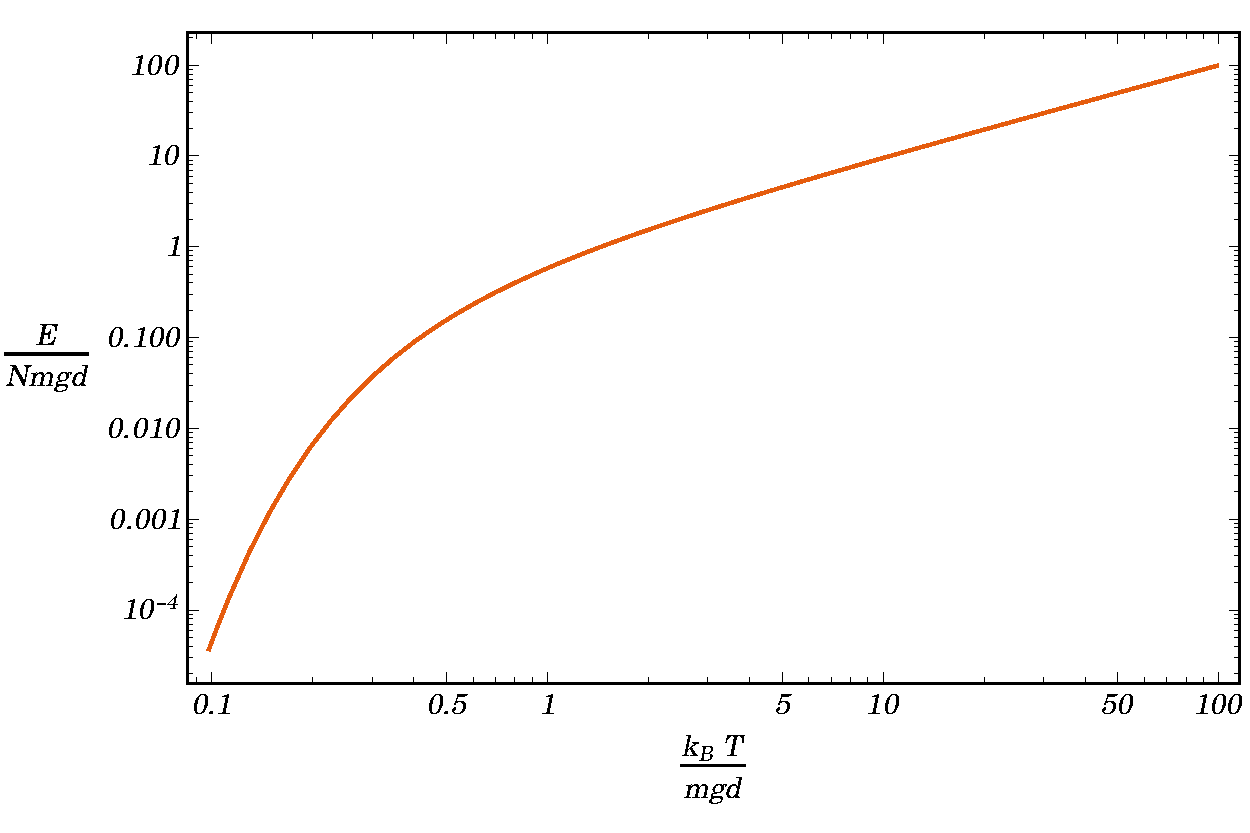
\includegraphics[width = 9cm, height = 6cm]{LogGravLatticeEnergy}
\caption{High temperature energy-temperature relationship for a one-dimensional lattice in a gravitational field plotted on a log-log scale.}
\label{loggravlattice}
\end{center}
\end{figure}
so the energy falls off exponentially. This is a general feature of a system with an energy gap, that is a finite gap in energy between the lowest energy and first excited states, because for temperatures much less than the energy of the gap there is a very low probability of exciting a particle above the gap so the system is approximately in its ground state. The different regimes of temperature dependence can clearly be seen in figure \ref{loggravlattice}. \bigskip\\
Another interesting quantity to study is the heat capacity which measures the increase in energy due to a set change in temperature. Explicitly, the heat capacity is given by,
\[ C = \pderiv{E}{T} = \frac{(mgd)^2}{k_B T^2} \frac{N e^{\frac{mgd}{k_B T}}}{(e^{\frac{mgd}{k_B T}} - 1)^2} = N k_B \left( \frac{T_c}{T} \right)^2 \frac{e^{T_c/T}}{(e^{T_c/T} - 1)^2} \]
The heat capacity tells us the same story. At high temperature, the heat capacity is approximately constant which is indicative of a gas like substance with linear energy-temperature dependence. However, near the critical temperature, the heat capacity drops to zero due to the relatively large amount of energy needed to make the jump across the gap to an excited state. \bigskip \\
The order of magnitude of the heat capacity $\sim N k_B$ is quite general. This gives us even more reason to call $k_B$ the conversion factor between microscopic energies and macroscopic energies since $k_B$ is the approximate heat capacity of a single atom of a system.  

\begin{figure}
\begin{center}
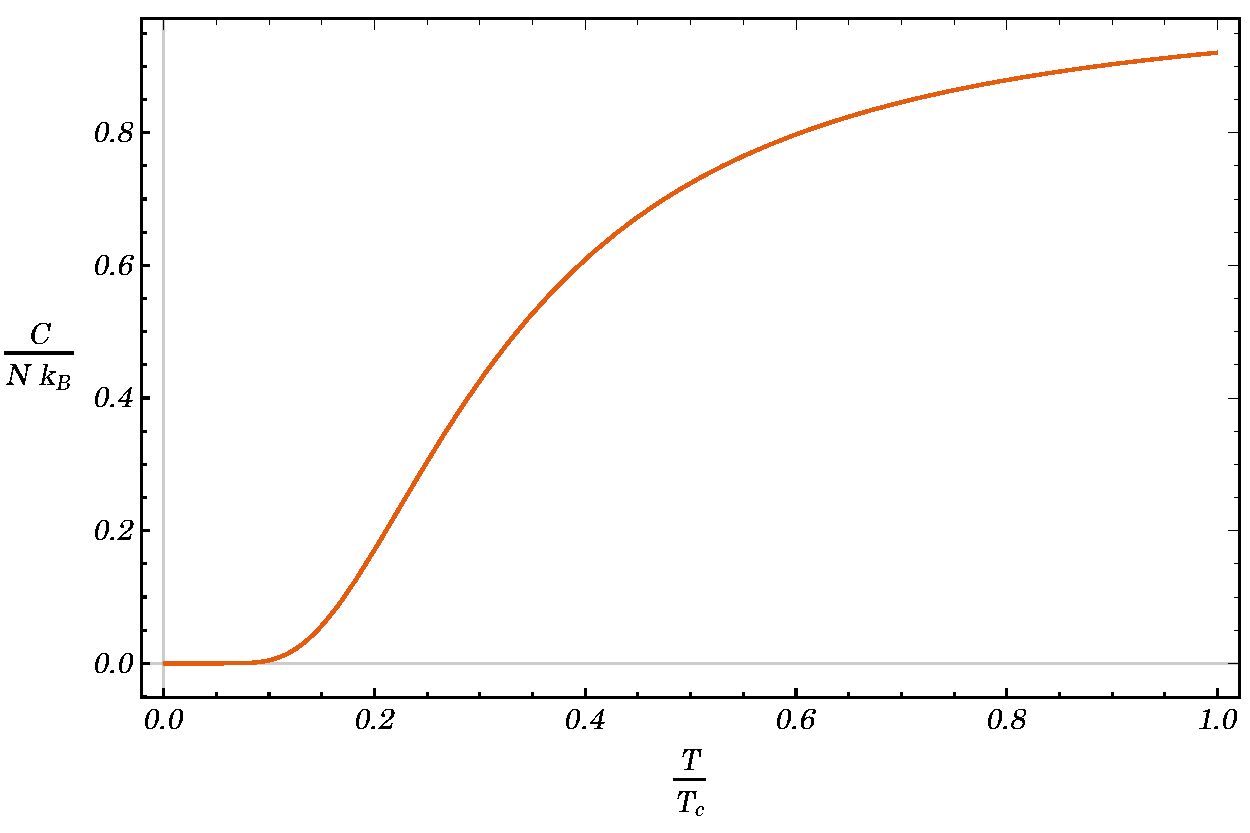
\includegraphics[width = 9cm, height = 6cm]{GravLatticeCapacity}
\caption{Heat capacity as a function of temperature for a one-dimensional lattice in a gravitational field.}
\label{capacitygravlattice}
\end{center}
\end{figure}

\subsection{Interacting Particles in a Lattice}

Now we will consider a somewhat more involved problem, interacting particles confined to a lattice in the tight binding approximation. Consider a lattice with $N$ spots and $N$ electrons filling these spots. However, more than one electron may inhabit the same lattice node but they give rise to a repulsive energy of $E_0(n - 1)$ where $n$ is the number of electrons in a single node. To simplify the book keeping we will take all the particles to be identical such that any reordering represents the same microstate\footnote{What exactly ``identical'' means is a very deep question which contains in it quite a lot of nontrivial physics. However, we will have to wait until the section on quantum statistical physics to fully understand what this means.}. Now let's calculate the partition function of this system. The number of overlapping electrons (the sum of $n - 1$ for each lattice node) is equal to the number of empty lattice nodes because the number of lattice points is equal to the number of electrons. Therefore, the number of states with energy $k E_0$ is given by the number of ways to choose $k$ empty lattice points times the number of ways to fill the remaining $N - k$ nodes times the number of ways to add the extra $k$ electrons to any of the $N - k$ filled nodes divided by $N!$ to 
\[ {N \choose k} (N - k)! (N - k)^k \frac{1}{N!} = \frac{N!}{k! (N - k)!} \frac{(N - k)!}{N!} (N - k)^k = \frac{(N - k)^k}{k!} \] 
(FIX THIS)

\section{Control Parameters and Pressure}

So far, we have only considered systems dependent on a single variable, the total energy.  However, systems become much more interesting when we have not just one but two variables to play with. We will now introduce other ``control'' parameters, macroscopic parameters which an experimenter can change freely. The most important control parameter\footnote{We have already considered parameters such as energy, temperature, and the number of particles or amount of material which may also be considered control parameters.} is the volume of the system. In this section, we will consider control parameters in general which will lead us to the Legendere transformation, conjugate thermodynamical variables, and the first of many uses of the Helmholtz free energy. 

\subsection{Adiabtic Processes}

The term adiabatic comes from the greek word ``\textgreek{<adi'abatos}'' meaning impassable which referes to a process impassable to the flow of energy. That is, an adiabatic process is one in which no heat is exchanged with the surroundings. However, in statistical mechanincs, the word adiabatic has a more specific meaning. An adiabatic process is slow (on the microscopic scale), transfers no heat, and is thermodynamically reversible. These conditions imply that an adiabatic process occurs at constant entropy which explains why they are somestimes known as isentropic. An adiabatic process is a carefully choosen idealization which captures the important features of the response of a system to a control parameter. We requre that an adiabatic process is ``slow'' such that the system can be assumed to have reached thermodynamical equilibrium at each instant during the the process. That is, the system continuously changes from one equilibrium state to another through a sequence of intermediate equilibium states. The requirement that the process be reversible and transfer no heat are imposed to isolate the effect on the energy and temperature of chaning the control parameter alone while keeping the entropy (which we have seen is related to the amount of heat added) constant. 
 
\subsection{Conjugate Variables}

Suppose our system and therefore the phase space $\phase$ depend on some control parameter $I$. Then, we can write our parition function for the equilibirum ensemble $Z(I)$ as a function of $I$. Therefore, the equilibrium energy becomes a function of $I$ and temperature via,
\[ E(T, I) = - \deriv{\log{Z(I)}}{\beta} \]
Suppose we adiabatically change $I$, how does the energy of the system change? It turns out that this dependence is a fundamental quantitity associated with the control parameter. We define $J$, the thermodynamical conjugate variable to $I$ by the change in energy with $C$ at constant entropy,
\[ J = - \cderiv{E}{I}{S} \]
Although this definition may seem pulled from nowhere, the reasons for it will become much more clear when concerete examples are discussed in the next section.
However, when we discuss the properties of a real material, we care a lot more about the temperature dependence which can be readily measured than the entropy dependence. Therefore, we would like to write this quantitiy without reference to the entropy. Consider the variables $E(T, I)$ and $S(T, I)$ as functions of the variables $T$ and $I$. We can write, in terms of our ``coordinate'' variables,
\[ \cderiv{E}{I}{S} = \cderiv{E}{I}{T} \cderiv{I}{I}{S} + \cderiv{E}{T}{I} \cderiv{T}{I}{S} \]
However, since $S$ is fixed in the process, 
\[ \d{S} = \cderiv{S}{I}{T} \d{I} + \cderiv{S}{T}{I} \d{T} = 0 \]
Therefore,
\[ \cderiv{T}{I}{S} = - \frac{\cderiv{S}{I}{T}}{\cderiv{S}{T}{I}} \]
so plugging in and noticing that $\cderiv{I}{I}{S} = 1$,
\[ \cderiv{E}{I}{S} = \cderiv{E}{I}{T} - \frac{\cderiv{E}{T}{I}}{\cderiv{S}{T}{I}}
 \cderiv{S}{I}{T} \]
However, at fixed $I$, 
\[ \cderiv{E}{T}{I} = \cderiv{E}{S}{I} \cderiv{S}{T}{I} \]
and thus,
\[ \cderiv{E}{I}{S} = \cderiv{E}{I}{T} - \cderiv{E}{S}{I}
 \cderiv{S}{I}{T} \]
However, by our definition of temperature, we know that, keeping control parameters fixed,
\[ T = \cderiv{E}{S}{I} \]
so we have,
\[\cderiv{E}{I}{S} = \cderiv{E}{I}{T} - T \cderiv{S}{I}{T} = \cderiv{(E - TS)}{I}{T} = \cderiv{F}{I}{T} \]
where I can bring $T$ inside the derivative because it is taken at constant $T$. Magically the free energy shows up. Finally, we have completed the original goal,
\[ J = - \cderiv{F}{I}{T} = \cderiv{k_B T \log{Z}}{I}{T} \]
We are starting to see the ubiquity of the Helmholltz free energy and just how much information is containted in the quantity $\log{Z}$. 

\subsection{Pressue and Volume}

Now lets apply these ideas to a more concrete senario, a system constrained in a box where our control parameter is $V$ the total volume of the box. It turns out that the conjugate variable to the volume is the pressure, in symbols,
\[ P = - \cderiv{E}{V}{S} = - \cderiv{F}{V}{T}  =\cderiv{k_B T \log{Z}}{V}{T} \]

(EXPLAIN WHY)

\subsection{An Example of Pressure}

\section{The Ideal Gas Law and Beyond}

Finally, we have the tools to apply our statistical mechanics machinery to a real problem, gas in a box. The power of statistical mechanics is not just that we will be able to quickly and cleanly derive the ideal gas law, there are many other methods to do that, it is how seamlessly we will be able to generalize the ideal gas law to interacting gases.

\subsection{Ideal Gases}

Consider a system of $N$ non-interating particles of mass $m$ in a box of volume $V$ assumed to be much much smaller than the dimensions of the box. A state in the $6N$ dimensional phase space is given by the positions and momenta of all these particles. Because there are no interactions and thus no potential energy, the energy of a state is simply given by the kinetic energy,
\[E(X) = \sum\limits_{i = 1}^N \frac{p_i^2}{2m} = \sum\limits_{i = j}^{3N} \frac{p_j^2}{2m}\]
 where $j$ runs over both the particles and the $x$, $y$, and $z$ components of the momenta.
Therefore, the partition function becomes,
\[ Z = \int \d{p_1} \d{p_2} \cdots \d{p_{3N}} \d{V_1} \d{V_2} \cdots \d{V_N} \: \: \exp{\left[- \beta \sum\limits_{j = 1}^{3N} \frac{p_j^2}{2m} \right]} \]
where we integrate over the position of each particle and the $3N$ coordinates of the momentum of each particle. Each integral over the volume simply gives a factor of $V$ and we can split up the integrals over $p_j$ as,
\[ Z = V^N \left[ \int_{-\infty}^{\infty} \d{p} \: e^{- \beta \frac{p^2}{2m}} \right]^{3N} = V^N  \left( \frac{2m\pi}{\beta} \right)^{\frac{3N}{2}} \]
where I have used the fact that\footnote{If you have never seen this before check out ``Gaussian integral'' on Wikipedia. The proof is very clever and worth reading.},
\[ \int_{-\infty}^{\infty} e^{-a u^2} \d{u} = \sqrt{\frac{\pi}{a}} \]
Now consider the quantity from which we can derive everything of interest,
\[ \log{Z} = N \log{V} - \frac{3 N}{2} \log{\beta} + \frac{3 N}{2} \log{2 m \pi} \]
Now we can read off the important quantities,
\[ E = - \deriv{\log{Z}}{\beta} = \frac{3 N}{2} \frac{1}{\beta} = \frac{3}{2} N k_B T\]
which gives us two famous results: the energy of a ideal gas is a function of temperature alone as is linear in temperature and the energy of an ideal gas is $\frac{1}{2} k_B T$ for each ``degree of freedom'' i.e. coordinate needed to specify the position of the system. Likewise,
\[ P = -\cderiv{F}{V}{T} = \cderiv{k_B T \log{Z}}{V}{T} = \frac{N k_B T}{V} \]
which rearranging,
\[ PV = N k_B T \]
is the famous ideal gas law. This is sometimes writen by chemists as,
\[ PV = n RT \]
where $R = 8.314 \: \mathrm{J} \, \mathrm{K}^{-1} \, \mathrm{mol}^{-1}$ is the gas constant and $n$ is the number of gas molecules in moles. Therefore, we see that $k_B = \frac{R}{1 \, \mathrm{mol}}$ gives the ratio between the macroscopic quantities and the microscopic ones by dividing by the usual size of a macroscopic system in terms of number of atoms. \bigskip\\
Furthermore, the average energy per particle is,
\[ \left<E_{particle} \right> = \frac{E}{N} = \frac{3}{2} k_B T = \frac{1}{2} m \left<v^2\right> \]
and therefore,
\[ v_{\mathrm{rms}} = \sqrt{\left< v^2 \right>} = \sqrt{\frac{3 k_B T}{m}} \]
where r.m.s. stands for root mean square which is a type of average defined by the square root of the average of the square i.e. $\sqrt{\left<v^2\right>}$. 

\subsection{The Maxwell-Boltzmann Distribution}

We can use the Boltzmann distribution to learn a bit more about the ensemble of an ideal gas. Specifically, we are interested in the distribution of velocities of particles in the gas. The Boltzmann distribution tells us  

\subsection{Non-Ideal Gases}

Using  Kinetic theory, it is not obvious how to generalize the ideal gas law to more complicated senarios involving interacting particles. However, in statistical mechanincs, all we need to do is alter the energy $E(X)$ associated to each state and crank out the results. For a complicated energy function however, this is easier said than done. 

\subsubsection{Particles in a Box with Gravity}

\subsubsection{Interacting Gases}

\subsubsection{Models of Real Gases}

\section{The Equipartition Theorem}

\subsection{Molecular Gases}

\subsection{Heat Capacity}

\subsection{The Failure of Classical Physics}

\subsection{A Quantum Statistical Gas}

\section{Some Further Phenomena} 

\subsection{Thermal Fluctuations}

\subsection{Phase Transitions}

\subsection{Negative Temperatures}

\section{Maxwell Relations}

\subsection{The Legendere Transformation}

\subsection{Enthalpy}

\subsection{Gibbs Free Energy}

\subsection{Deriving the Maxwell Relations}

\section{Magnetization}

\subsection{Polarization and Magnetization}

\subsubsection{Same Idea Works in Quantum Mechanics}

\subsection{Magnetization of Uncoupled Spins}

\subsection{Coupled Spins}

\subsection{The Ising Model}

\subsection{Magnetic Phase Transitions}

\section{The Grand Canonical Ensemble}

\subsection{Microcanonical and Canonical Ensembles}

\subsection{The Grand Partition Function}

\subsection{The Grand Potential}

\subsection{The Chemical Potential}

\subsection{Applications of the Grand Ensemble}

\section{Quantum Statistical Mechanics}

\subsection{Bose-Einstein Statistics}

\subsection{Fermi-Dirac Statistics}

\subsection{Comparision to Maxwell-Boltzmann}

\section{The Magnetism of Matter}

\subsection{Ferromagnetism}

\end{document}

